\documentclass{article}
\usepackage{amsmath}
\usepackage{amssymb}
\usepackage{geometry}
\geometry{a4paper, margin=1in}
\usepackage{graphicx}
\usepackage{verbatim}
\usepackage{varwidth}
\usepackage{fancybox, verbatimbox}
\usepackage{listings}



% Custom Course Number
\newcommand{\coursenumber}{AME 5763}

\begin{document}

% Title Page on its own page without extra blank pages
\begin{titlepage}
    \centering
    {\LARGE \bfseries Exam 2 \par}
    \vspace{1cm}
    {\Large Blake Johnson \par}
    \vspace{0.5cm}
    {\Large \coursenumber \par}
    \vfill
    {\large \today \par}
\end{titlepage}

\newpage  % Ensures no extra blank page

\section*{Problem 1}

Consider an element shown in Fig. 1 with a quadratic displacement field \( u(x) = a_1 + a_2 x + a_3 x^2 \).

\begin{figure}[h!]
    \centering
    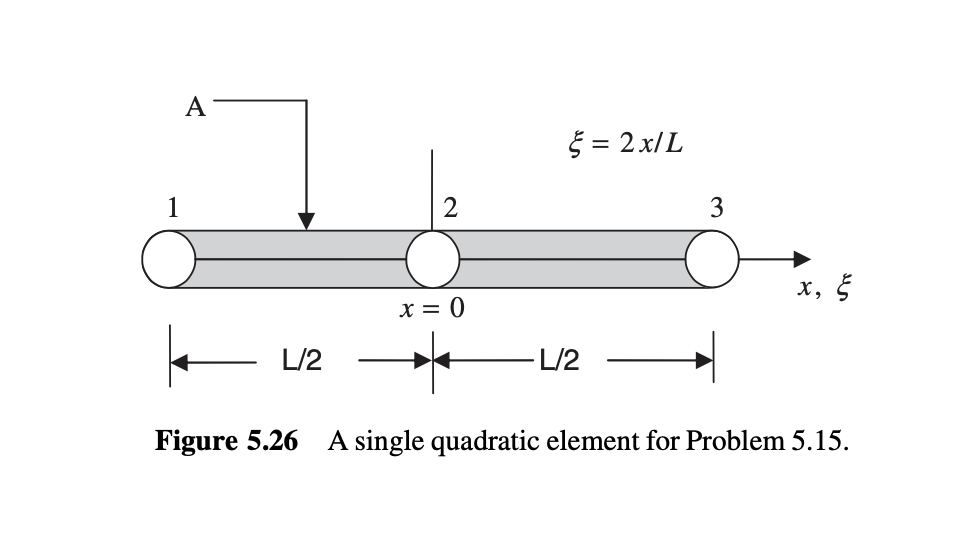
\includegraphics[width=0.5\textwidth]{figure_1.png}  % Replace with your image file name
    \caption{Problem 1}
    \label{fig:element}
\end{figure}

\begin{enumerate}
    \item[(a)] (10 points) Express the displacement field in terms of the nodal displacements \( d_1 \), \( d_2 \), and \( d_3 \). (Hint: Use the quadratic interpolants in the local coordinate \( \xi \).)
    
    \item[(b)] (5 points) For a linear body force field \( b(\xi) = b_1 \frac{1}{2}(1 - \xi) + b_3 \frac{1}{2}(1 + \xi) \), show that the external force matrix is given by 
    \[
    \mathbf{f}_e = L \begin{bmatrix} b_1 & 2(b_1 + b_3) & b_3 \end{bmatrix}^T.
    \]
    
    \item[(c)] (5 points) Develop the \( \mathbf{B}_E \) matrix such that \( \epsilon = \frac{du}{dx} = \mathbf{B}_E \mathbf{d}_E \), where \( \mathbf{d}_E = \begin{bmatrix} u_1 & u_2 & u_3 \end{bmatrix}^T \).
    
    \item[(d)] (5 points) Use one three-node quadratic element to solve, by finite elements, the differential equation \( E \frac{d^2 u}{dx^2} = -b(x) = -c x \) with boundary conditions \( u\left(-\frac{L}{2}\right) = u\left(\frac{L}{2}\right) = 0.0 \).
    
    \item[(e)] (5 points) Compare the FEM results to the exact solution for \( u(x) \) and \( \sigma(x) \).
\end{enumerate}

\subsection*{Given values for problem 1}

\begin{equation}
    u_{x} = a_{1} + a_{2}x + a_{3}x^{2}
    \label{eq:u(x)}
\end{equation}

\begin{equation}
    \xi = \frac{2x}{L}
    \label{eq:xi}
\end{equation}

\begin{equation}
    \xi_{1} = -1
    \label{eq:xi_1}
\end{equation}

\begin{equation}
    \xi_{2} = 0
    \label{eq:xi_2}
\end{equation}

\begin{equation}
    \xi_{3} = 1
    \label{eq:xi_3}
\end{equation}

\begin{equation}
    N_1 = \frac{(x - x_2)(x-x_3)}{(x_1 - x_2)(x_1 - x_2)}
    \label{eq:N_1}
\end{equation}

\begin{equation}
    N_2 = \frac{(x - x_1)(x - x_3)}{(x_2 - x_1)(x_2 - x_3)}
    \label{eq:N_2}
\end{equation}

\begin{equation}
    N_3 = \frac{(x - x_1)(x - x_2)}{(x_3 - x_1)(x_3 - x_2)}
    \label{eq:N_3}
\end{equation}

\begin{equation}
    f_{\Omega} = \int_{x_1}^{x_2} N^{eT}b dx
    \label{eq:eforce}
\end{equation}

\begin{equation}
    J = \frac{dx}{d\xi}
    \label{eq:jacobian}
\end{equation}

\subsection*{a.$)$ Express the displacement field in terms of the nodal displacements $d_1$,$d_2$,$d_3$.}

\subsubsection*{Lagrange Interpolations of the Shape Functions}
Let's find the shape functions with respect to $\xi$ by substituting equations \eqref{eq:xi_1}, \eqref{eq:xi_2}, 
and \eqref{eq:xi_3} into equations \eqref{eq:N_1}, \eqref{eq:N_2}, and \eqref{eq:N_3}.

\[
    N_1(\xi) = \frac{(\xi - 0)(\xi - 1)}{(-1 - 0)(-1 - 1)} = \frac{\xi (1 - \xi)}{2} = \frac{1}{2} \xi (1 - \xi)
\]
\[
    N_2(\xi) = \frac{(\xi + 1)(\xi - 1)}{(0 + 1)(0 - 1)} = 1 - \xi^2
\]
\[
    N_3(\xi) = \frac{(\xi + 1)(\xi - 0)}{(1 + 1)(1 - 0)} = \frac{\xi (1 + \xi)}{2} = \frac{1}{2} \xi (1 + \xi)
\]
These values can be confimed by the interpolation property and the partition of unity. The interpolation property states that
the value of each shape function is equal to one at its node and equal to zero at all other nodes.
\begin{equation*}
    N_i(\xi_j) = \delta_{ij}
\end{equation*}

The partition unity states that the sum of all the shape functions should equal one.
So we can confirm these values.

\subsubsection*{Verification for \( N_1(\xi) \)}

\begin{align*}
    N_1(-1) &= \frac{1}{2}(-1)(-1 - 1) \\
            &= \frac{1}{2}(-1)(-2) \\
            &= \frac{1}{2} \cdot 2 \\
            &= \frac{2}{2} \\
            &= 1
\end{align*}

\begin{align*}
    N_1(0) &= \frac{1}{2}(0)(0 - 1) \\
           &= \frac{1}{2} \cdot 0 \\
           &= 0
\end{align*}

\begin{align*}
    N_1(1) &= \frac{1}{2}(1)(1 - 1) \\
           &= \frac{1}{2} \cdot 0 \\
           &= 0
\end{align*}

\subsubsection*{Verification for \( N_2(\xi) \)}

\begin{align*}
    N_2(-1) &= 1 - (-1)^2 \\
            &= 1 - 1 \\
            &= 0
\end{align*}

\begin{align*}
    N_2(0) &= 1 - (0)^2 \\
           &= 1 - 0 \\
           &= 1
\end{align*}

\begin{align*}
    N_2(1) &= 1 - (1)^2 \\
           &= 1 - 1 \\
           &= 0
\end{align*}

\subsubsection*{Verification for \( N_3(\xi) \)}

\begin{align*}
    N_3(-1) &= \frac{1}{2}(-1)(-1 + 1) \\
            &= \frac{1}{2}(-1)(0) \\
            &= 0
\end{align*}

\begin{align*}
    N_3(0) &= \frac{1}{2}(0)(0 + 1) \\
           &= \frac{1}{2} \cdot 0 \\
           &= 0
\end{align*}

\begin{align*}
    N_3(1) &= \frac{1}{2}(1)(1 + 1) \\
           &= \frac{1}{2}(1)(2) \\
           &= \frac{2}{2} \\
           &= 1
\end{align*}
This confirms the shape functions for each node.

\subsubsection*{Interpolated Function}
If \( d_1 \), \( d_2 \), and \( d_3 \) are the values of the distribution \( u \) at the nodes, the quadratic interpolation \( u(\xi) \) over the element in local coordinates can be expressed as:

\begin{equation}
    u(\xi) = N_1(\xi) d_1 + N_2(\xi) d_2 + N_3(\xi) d_3
    \label{eq:displacement}
\end{equation}

Substituting the equations $N_1$, $N_2$, and $N_3$ into the function we get.

\begin{equation}
    u(\xi) = \frac{1}{2} \xi (\xi - 1) d_1 + (1 - \xi^2) d_2 + \frac{1}{2} \xi (\xi + 1) d_3
\end{equation}

\subsubsection*{Substitute $\xi$}
The problem gives us the value for $ \xi = \frac{2x}{L} $. So to finalize the displacement field we can substitute and simplify.

\begin{equation}
    u(\xi) = \frac{1}{2} \xi (\xi - 1) d_1 + (1 - \xi^2) d_2 + \frac{1}{2} \xi (\xi + 1) d_3
\end{equation}

Substituting \( \xi = \frac{2x}{L} \):

\begin{align*}
    u(x) &= \frac{1}{2} \left( \frac{2x}{L} \right) \left( \frac{2x}{L} - 1 \right) d_1 + \left( 1 - \left( \frac{2x}{L} \right)^2 \right) d_2 + \frac{1}{2} \left( \frac{2x}{L} \right) \left( \frac{2x}{L} + 1 \right) d_3 \\
    &= \frac{1}{2} \cdot \frac{2x}{L} \cdot \frac{2x - L}{L} \, d_1 + \left( 1 - \frac{4x^2}{L^2} \right) d_2 + \frac{1}{2} \cdot \frac{2x}{L} \cdot \frac{2x + L}{L} \, d_3 \\
    &= \frac{2x (2x - L)}{2L^2} \, d_1 + \left( \frac{L^2 - 4x^2}{L^2} \right) d_2 + \frac{2x (2x + L)}{2L^2} \, d_3 \\
    &= \frac{2x^2 - xL}{L^2} \, d_1 + \frac{L^2 - 4x^2}{L^2} \, d_2 + \frac{2x^2 + xL}{L^2} \, d_3\\
    &=  \left(\frac{2x^2 - xL}{L^2} \right) \, d_1 + \left( \frac{L^2 - 4x^2}{L^2} \right) \, d_2 + \left( \frac{2x^2 + xL}{L^2} \right) \, d_3
\end{align*}

Thus, the simplified form of \( u(x) \) is:

\begin{equation*}
    u(x) = \frac{1}{L^2}\left[ x(2x-L)  \, d_1 + \left( L^{2}-4x^2 \right) \, d_2 + \left( x(2x+L) \right) \, d_3 \right]
\end{equation*}



%%%%%%%%%%

\newpage
\subsection*{ b.$)$}

For a linear body force field $ b(\xi) = b_1 \frac{1}{2}(1 - \xi) + b_3 \frac{1}{2}(1 + \xi)$ , show that the external force matrix is given by 
\[
\mathbf{f}_e = L \begin{bmatrix} b_1 & 2(b_1 + b_3) & b_3 \end{bmatrix}^T.
\]


\subsubsection*{The External Force Matrix}
The external force matrix $f_{\Omega}$ can be calculated using \ref{eq:eforce} when the function is in terms of x.
However the problem we are give is in terms of $\xi$ and so we need to adjust for that. We do this by using the Jacobian Term.

\subsubsection*{The Jacobian}
The Jacobian can be calculated with \ref{eq:jacobian}. The jacobian is the derivative of x with respect to $\xi$. The problem gives us the 
length of the element which is L. Additionally, we are using -1 and 1 as the values for $\xi_1$ and $\xi_3$ respectively. So the Jacobian can
be calculated as:
\begin{equation*}
    J = \frac{\Delta x}{\Delta \xi} = \frac{(L-0)}{(1-(-1))} = \frac{L}{2}
\end{equation*}

\subsubsection*{Calculating the External Force Matrix at Node 1}

To compute \( f_1 \), we start with the integral expression:

\begin{equation}
    f_1 = \int_{-1}^{1} N_1(\xi) \left( b_1 \frac{1}{2}(1 - \xi) + b_3 \frac{1}{2}(1 + \xi) \right) \frac{L}{2} \, d\xi
\end{equation}

where \( N_1(\xi) = \frac{1}{2} \xi (\xi - 1) \). Substituting \( N_1(\xi) \) into the equation, we have:

\begin{align*}
    f_1 &= \int_{-1}^{1} \frac{1}{2} \xi (\xi - 1) \left( b_1 \frac{1}{2}(1 - \xi) + b_3 \frac{1}{2}(1 + \xi) \right) \frac{L}{2} \, d\xi \\
    &= \frac{L}{8} \int_{-1}^{1} \xi (\xi - 1) \left( b_1(1 - \xi) + b_3(1 + \xi) \right) d\xi \\
    &= \frac{L}{8} \int_{-1}^{1} \left( b_1 \xi (\xi - 1)(1 - \xi) + b_3 \xi (\xi - 1)(1 + \xi) \right) d\xi
\end{align*}

Now we expand each term:

\begin{align*}
    f_1 &= \frac{L}{8} \int_{-1}^{1} \left( b_1 \xi (\xi^2 - 2\xi + 1) + b_3 \xi (\xi^2 - 1) \right) d\xi \\
    &= \frac{L}{8} \int_{-1}^{1} \left( b_1 (\xi^3 - 2\xi^2 + \xi) + b_3 (\xi^3 - \xi) \right) d\xi \\
    &= \frac{L}{8} \int_{-1}^{1} \left( (b_1 + b_3) \xi^3 - (2b_1) \xi^2 + (b_1 - b_3) \xi \right) d\xi
\end{align*}

Now we integrate each term over \([-1, 1]\):

\begin{align*}
    f_1 &= \frac{L}{8} \left[ (b_1 + b_3) \int_{-1}^{1} \xi^3 \, d\xi - 2b_1 \int_{-1}^{1} \xi^2 \, d\xi + (b_1 - b_3) \int_{-1}^{1} \xi \, d\xi \right]
\end{align*}

Evaluating each integral:

\begin{align*}
    \int_{-1}^{1} \xi^3 \, d\xi &= 0, \\
    \int_{-1}^{1} \xi^2 \, d\xi &= \frac{2}{3}, \\
    \int_{-1}^{1} \xi \, d\xi &= 0.
\end{align*}

Substituting these values back:

\begin{align*}
    f_1 &= \frac{L}{8} \left[ 0 - 2b_1 \cdot \frac{2}{3} + 0 \right] \\
    &= \frac{L}{8} \cdot \frac{-4}{3} b_1 \\
    &= \frac{-L}{6} b_1.
\end{align*}

Thus, the simplified result for \( f_1 \) is:

\begin{equation}
    f_1 = \frac{L}{6} b_1
\end{equation}


\subsubsection*{Calculating the External Force Matrix at Node 2}

To compute \( f_2 \), we start with the integral expression:

\begin{equation}
    f_2 = \int_{-1}^{1} N_2(\xi) \left( b_1 \frac{1}{2}(1 - \xi) + b_3 \frac{1}{2}(1 + \xi) \right) \frac{L}{2} \, d\xi
\end{equation}

where \( N_2(\xi) = 1 - \xi^2 \). Substituting \( N_2(\xi) \) into the equation, we have:

\begin{align*}
    f_2 &= \int_{-1}^{1} \left(1 - \xi^2\right) \left( b_1 \frac{1}{2}(1 - \xi) + b_3 \frac{1}{2}(1 + \xi) \right) \frac{L}{2} \, d\xi \\
    &= \frac{L}{2} \int_{-1}^{1} \left(1 - \xi^2\right) \left( \frac{b_1}{2}(1 - \xi) + \frac{b_3}{2}(1 + \xi) \right) d\xi \\
    &= \frac{L}{4} \int_{-1}^{1} \left( (1 - \xi^2)(b_1(1 - \xi) + b_3(1 + \xi)) \right) d\xi
\end{align*}

Now we expand \( (1 - \xi^2)(b_1(1 - \xi) + b_3(1 + \xi)) \):

\begin{align*}
    f_2 &= \frac{L}{4} \int_{-1}^{1} \left( b_1(1 - \xi)(1 - \xi^2) + b_3(1 + \xi)(1 - \xi^2) \right) d\xi \\
    &= \frac{L}{4} \int_{-1}^{1} \left( b_1 (1 - \xi - \xi^2 + \xi^3) + b_3 (1 + \xi - \xi^2 - \xi^3) \right) d\xi \\
    &= \frac{L}{4} \int_{-1}^{1} \left( (b_1 + b_3) - (b_1 - b_3)\xi - (b_1 + b_3)\xi^2 + (b_1 - b_3)\xi^3 \right) d\xi
\end{align*}

Now we integrate each term individually over \([-1, 1]\):

\begin{align*}
    f_2 &= \frac{L}{4} \left[ (b_1 + b_3) \int_{-1}^{1} 1 \, d\xi - (b_1 - b_3) \int_{-1}^{1} \xi \, d\xi - (b_1 + b_3) \int_{-1}^{1} \xi^2 \, d\xi + (b_1 - b_3) \int_{-1}^{1} \xi^3 \, d\xi \right]
\end{align*}

Evaluating each integral:

\begin{align*}
    \int_{-1}^{1} 1 \, d\xi &= 2, \\
    \int_{-1}^{1} \xi \, d\xi &= 0, \\
    \int_{-1}^{1} \xi^2 \, d\xi &= \frac{2}{3}, \\
    \int_{-1}^{1} \xi^3 \, d\xi &= 0.
\end{align*}

Substituting these values back:

\begin{align*}
    f_2 &= \frac{L}{4} \left[ (b_1 + b_3) \cdot 2 - (b_1 + b_3) \cdot \frac{2}{3} \right] \\
    &= \frac{L}{4} \left( 2(b_1 + b_3) - \frac{2}{3}(b_1 + b_3) \right) \\
    &= \frac{L}{4} \cdot \frac{4}{3} (b_1 + b_3) \\
    &= \frac{L}{3} (b_1 + b_3)
\end{align*}

Thus, the simplified result for \( f_2 \) is:

\begin{equation}
    f_2 = \frac{L}{6} [2(b_1 + b_3)]
\end{equation}


\subsubsection*{Calculating the External Force Matrix at Node 3}

To compute \( f_3 \), we start with the integral expression:

\begin{equation}
    f_3 = \int_{-1}^{1} N_3(\xi) \left( b_1 \frac{1}{2}(1 - \xi) + b_3 \frac{1}{2}(1 + \xi) \right) \frac{L}{2} \, d\xi
\end{equation}

where \( N_3(\xi) = \frac{1}{2} \xi (1 + \xi) \). Substituting \( N_3(\xi) \) into the equation, we have:

\begin{align*}
    f_3 &= \int_{-1}^{1} \frac{1}{2} \xi (1 + \xi) \left( b_1 \frac{1}{2}(1 - \xi) + b_3 \frac{1}{2}(1 + \xi) \right) \frac{L}{2} \, d\xi \\
    &= \frac{L}{8} \int_{-1}^{1} \xi (1 + \xi) \left( b_1(1 - \xi) + b_3(1 + \xi) \right) d\xi \\
    &= \frac{L}{8} \int_{-1}^{1} \left( b_1 \xi (1 + \xi)(1 - \xi) + b_3 \xi (1 + \xi)^2 \right) d\xi
\end{align*}

Now we expand each term:

\begin{align*}
    f_3 &= \frac{L}{8} \int_{-1}^{1} \left( b_1 \xi (1 - \xi^2) + b_3 \xi (1 + 2\xi + \xi^2) \right) d\xi \\
    &= \frac{L}{8} \int_{-1}^{1} \left( b_1 (\xi - \xi^3) + b_3 (\xi + 2\xi^2 + \xi^3) \right) d\xi \\
    &= \frac{L}{8} \int_{-1}^{1} \left( (b_1 + b_3) \xi + 2 b_3 \xi^2 + (b_3 - b_1) \xi^3 \right) d\xi
\end{align*}

Now we integrate each term over \([-1, 1]\):

\begin{align*}
    f_3 &= \frac{L}{8} \left[ (b_1 + b_3) \int_{-1}^{1} \xi \, d\xi + 2 b_3 \int_{-1}^{1} \xi^2 \, d\xi + (b_3 - b_1) \int_{-1}^{1} \xi^3 \, d\xi \right]
\end{align*}

Evaluating each integral:

\begin{align*}
    \int_{-1}^{1} \xi \, d\xi &= 0, \\
    \int_{-1}^{1} \xi^2 \, d\xi &= \frac{2}{3}, \\
    \int_{-1}^{1} \xi^3 \, d\xi &= 0.
\end{align*}

Substituting these values back:

\begin{align*}
    f_3 &= \frac{L}{8} \left[ (b_1 + b_3) \cdot 0 + 2 b_3 \cdot \frac{2}{3} + (b_3 - b_1) \cdot 0 \right] \\
    &= \frac{L}{8} \cdot \frac{4}{3} b_3 \\
    &= \frac{L}{6} b_3
\end{align*}

Thus, the simplified result for \( f_3 \) is:

\begin{equation}
    f_3 = \frac{L}{6} b_3
\end{equation}

\subsubsection*{Putting the External Force in Matrix form}
Now that we have the External Force for all three nodes we can put it in matrix form to confirm the values given:

The force vector \( \mathbf{f}_e \) in matrix form is:

\begin{equation}
    \mathbf{f}_e = \begin{bmatrix} f_1 \\ f_2 \\ f_3 \end{bmatrix} = \frac{L}{6} \begin{bmatrix} b_1 \\ 2(b_1 + b_3) \\ b_3 \end{bmatrix}
\end{equation}

\newpage
\subsection*{c.$)$}
Develop the \( \mathbf{B}_E \) matrix such that:

\begin{equation}
    \epsilon = \frac{du}{dx} = \mathbf{B}_E \, \mathbf{d}_E
\end{equation}

where

\begin{equation}
    \mathbf{d}_E = \begin{bmatrix} u_1 \\ u_2 \\ u_3 \end{bmatrix}^T
\end{equation}

The displacement field can be represented in local notation from \ref{eq:displacement}.
We are told that $\epsilon = \frac{du}{dx}$ however our function is in terms of $\xi$.
So to get $\frac{du}{dx}$ from a function that is dependent on $\xi$ we can use the chain rule:

\begin{equation}
    \epsilon = \frac{du}{dx} = \frac{dN_1}{dx} u_1 + \frac{dN_2}{dx} u_2 + \frac{dN_3}{dx} u_3
\end{equation}

becomes:
\begin{equation}
    \epsilon = \frac{du}{dx} = \frac{dN_1}{d\xi} \frac{d\xi}{dx} u_1 + \frac{dN_2}{d\xi} \frac{d\xi}{dx} u_2 + \frac{dN_3}{d\xi} \frac{d\xi}{dx} u_3
\end{equation}

The Jacobian \ref{eq:jacobian} shows that $\frac{d\xi}{dx} = \frac{L}{2}$ so we just need to find $\frac{dN}{d\xi}$.

\subsubsection*{Calculate $\frac{dN}{d\xi}$}

\subsubsection*{Shape Functions and Their Derivatives}

\subsubsection*{1. Shape Function \( N_1(\xi) \)}

\begin{align*}
    N_1(\xi) &= \frac{1}{2} \xi (\xi - 1) \\
             &= \frac{1}{2} \xi^2 - \frac{1}{2} \xi
\end{align*}

Taking the derivative with respect to \( \xi \):

\begin{align*}
    \frac{dN_1}{d\xi} &= \frac{d}{d\xi} \left( \frac{1}{2} \xi^2 - \frac{1}{2} \xi \right) \\
                       &= \frac{1}{2} (2\xi) - \frac{1}{2} \\
                       &= \xi - \frac{1}{2}
\end{align*}

\subsubsection*{2. Shape Function \( N_2(\xi) \)}

\begin{align*}
    N_2(\xi) &= 1 - \xi^2
\end{align*}

Taking the derivative with respect to \( \xi \):

\begin{align*}
    \frac{dN_2}{d\xi} &= \frac{d}{d\xi} (1 - \xi^2) \\
                       &= -2\xi
\end{align*}

\subsubsection*{3. Shape Function \( N_3(\xi) \)}

\begin{align*}
    N_3(\xi) &= \frac{1}{2} \xi (\xi + 1) \\
             &= \frac{1}{2} \xi^2 + \frac{1}{2} \xi
\end{align*}

Taking the derivative with respect to \( \xi \):

\begin{align*}
    \frac{dN_3}{d\xi} &= \frac{d}{d\xi} \left( \frac{1}{2} \xi^2 + \frac{1}{2} \xi \right) \\
                       &= \frac{1}{2} (2\xi) + \frac{1}{2} \\
                       &= \xi + \frac{1}{2}
\end{align*}

Now we can multiply it by the Jacobian and get our $\epsilon$

\subsection*{Derivatives of Shape Functions with Respect to \( x \)}

We want to calculate \( \frac{dN_i}{dx} \) for each shape function \( N_i(\xi) \) using the chain rule:

\[
\frac{dN_i}{dx} = \frac{dN_i}{d\xi} \cdot \frac{L}{2}
\]

\subsection*{Derivatives of Shape Functions with Respect to \( x \)}

Using the chain rule, each derivative \( \frac{dN_i}{dx} \) can be expressed as:

\[
\frac{dN_i}{dx} = \frac{dN_i}{d\xi} \cdot \frac{2}{L}
\]

For each shape function:

1. **For \( N_1(\xi) \):**
   \[
   \frac{dN_1}{d\xi} = \xi - \frac{1}{2} \Rightarrow \frac{dN_1}{dx} = \frac{2}{L} \left( \xi - \frac{1}{2} \right)
   \]

2. **For \( N_2(\xi) \):**
   \[
   \frac{dN_2}{d\xi} = -2\xi \Rightarrow \frac{dN_2}{dx} = -\frac{4\xi}{L}
   \]

3. **For \( N_3(\xi) \):**
   \[
   \frac{dN_3}{d\xi} = \xi + \frac{1}{2} \Rightarrow \frac{dN_3}{dx} = \frac{2}{L} \left( \xi + \frac{1}{2} \right)
   \]

\subsection*{Constructing the \( \mathbf{B}_e \) Matrix}

Using the derivatives calculated above, we can now construct the \( \mathbf{B}_e \) matrix:

\begin{equation}
    \mathbf{B}_e = \begin{bmatrix} \frac{2}{L} \left( \xi - \frac{1}{2} \right) & -\frac{4\xi}{L} & \frac{2}{L} \left( \xi + \frac{1}{2} \right) \end{bmatrix}
\end{equation}

This matrix \( \mathbf{B}_e \) now relates the nodal displacement vector \( \mathbf{d}_e \) to the strain \( \epsilon \) within the element:

\begin{equation}
    \epsilon = \mathbf{B}_e \, \mathbf{d}_e
\end{equation}

where

\[
\mathbf{d}_e = \begin{bmatrix} u_1 \\ u_2 \\ u_3 \end{bmatrix}
\]

\newpage
\subsection*{d.$)$}
Calculate the element stiffness matrix.


\subsubsection*{1. Element Stiffness Matrix Definition}

The element stiffness matrix \( \mathbf{K}^e \) for a one-dimensional bar element in the finite element method is expressed as:

\begin{equation}
    \mathbf{K}^e = \int_{-1}^{1} (\mathbf{B}^e)^T E A \, \mathbf{B}^e \, J \, d\xi
\end{equation}

where:
\begin{itemize}
    \item \( \mathbf{B}^e \) is the matrix of shape function derivatives, relating strain to nodal displacements,
    \item \( E \) is Young’s modulus,
    \item \( A \) is the cross-sectional area,
    \item \( J = \frac{L}{2} \) is the Jacobian, which converts the integral in the natural coordinate \( \xi \) to the physical length.
\end{itemize}

\subsubsection*{2. Substituting \( \mathbf{B}^e \) and the Jacobian}

The \( \mathbf{B}^e \) matrix, as derived previously, is:

\begin{equation}
    \mathbf{B}^e = \begin{bmatrix} \frac{2}{L} \left( \xi - \frac{1}{2} \right) & -\frac{4\xi}{L} & \frac{2}{L} \left( \xi + \frac{1}{2} \right) \end{bmatrix}
\end{equation}

Now, \( \mathbf{K}^e \) can be expressed as:

\begin{equation}
    \mathbf{K}^e = \int_{-1}^{1} (\mathbf{B}^e)^T E A \, \mathbf{B}^e \cdot \frac{L}{2} \, d\xi
\end{equation}

The \( \frac{L}{2} \) factor comes from the Jacobian \( J \).

\subsubsection*{3. Setting Up the Integral}

Expanding \( \mathbf{K}^e \), we have:

\begin{equation}
    \mathbf{K}^e = \frac{E A}{L} \int_{-1}^{1} (\mathbf{B}^e)^T \mathbf{B}^e \, d\xi
\end{equation}


%%%%%%%

\subsubsection*{3. Setting Up the Integral and Performing the Calculation}

Expanding \( \mathbf{K}^e \) in terms of the \( \mathbf{B}^e \) matrix, we have:

\[
    \mathbf{K}^e = \frac{E A}{L} \int_{-1}^{1} (\mathbf{B}^e)^T \mathbf{B}^e \, d\xi
\]

Given:

\[
    \mathbf{B}^e = \begin{bmatrix} \frac{2}{L} \left( \xi - \frac{1}{2} \right) & -\frac{4\xi}{L} & \frac{2}{L} \left( \xi + \frac{1}{2} \right) \end{bmatrix}
\]

we can calculate \( (\mathbf{B}^e)^T \mathbf{B}^e \) component-wise:

1. Calculating the first term:
   \[
   \left( \frac{2}{L} \left( \xi - \frac{1}{2} \right) \right)^2 = \frac{4}{L^2} \left( \xi^2 - \xi + \frac{1}{4} \right)
   \]

2. Calculating the second term:
   \[
   \left( -\frac{4\xi}{L} \right)^2 = \frac{16\xi^2}{L^2}
   \]

3. Calculating the third term:
   \[
   \left( \frac{2}{L} \left( \xi + \frac{1}{2} \right) \right)^2 = \frac{4}{L^2} \left( \xi^2 + \xi + \frac{1}{4} \right)
   \]

4. Expanding cross terms: Calculate cross terms such as \( \left( \frac{2}{L} \left( \xi - \frac{1}{2} \right) \right) \left( -\frac{4\xi}{L} \right) \):
   \[
   \frac{2}{L} \left( \xi - \frac{1}{2} \right) \cdot \left( -\frac{4\xi}{L} \right) = -\frac{8\xi}{L^2} \left( \xi - \frac{1}{2} \right) = -\frac{8}{L^2} \left( \xi^2 - \frac{\xi}{2} \right)
   \]

Summing these terms, we set up the integral:

\[
    \mathbf{K}^e = \frac{E A}{L} \int_{-1}^{1} \begin{bmatrix} \frac{4}{L^2} \left( \xi^2 - \xi + \frac{1}{4} \right) & -\frac{8}{L^2} \left( \xi^2 - \frac{\xi}{2} \right) & \frac{4}{L^2} \left( \xi^2 + \xi + \frac{1}{4} \right) \\ -\frac{8}{L^2} \left( \xi^2 - \frac{\xi}{2} \right) & \frac{16 \xi^2}{L^2} & -\frac{8}{L^2} \left( \xi^2 + \frac{\xi}{2} \right) \\ \frac{4}{L^2} \left( \xi^2 + \xi + \frac{1}{4} \right) & -\frac{8}{L^2} \left( \xi^2 + \frac{\xi}{2} \right) & \frac{4}{L^2} \left( \xi^2 - \xi + \frac{1}{4} \right) \end{bmatrix} d\xi
\]

Integrating term-by-term over \([-1, 1]\):

Each term can be evaluated using standard integral values for \(\int_{-1}^{1} \xi^2 \, d\xi = \frac{2}{3}\), \(\int_{-1}^{1} \xi \, d\xi = 0\), and \(\int_{-1}^{1} 1 \, d\xi = 2\).

I ran the integration in python but I am having trouble incorporating it in the pdf. The final results then simplified to:

\begin{equation}
    \mathbf{K}^e = \frac{A E}{3 L} \begin{bmatrix} 7 & -8 & 1 \\ -8 & 16 & -8 \\ 1 & -8 & 7 \end{bmatrix}
\end{equation}

%%%%%%


\subsubsection*{Final Stiffness Matrix}

The element stiffness matrix is:

\begin{equation}
    \mathbf{K}^e = \frac{A E}{3 L} \begin{bmatrix} 7 & -8 & 1 \\ -8 & 16 & -8 \\ 1 & -8 & 7 \end{bmatrix}
\end{equation}

This matrix can now be used in your finite element model to relate nodal forces to nodal displacements.

\newpage
\subsection*{e.$)$}

Use one three-node quadratic element to solve, by finite elements, the differential equation:

\[
E \frac{d^2 u}{dx^2} = -b(x) = -cx
\]

with boundary conditions:

\[
u\left(-\frac{L}{2}\right) = 0 \quad \text{and} \quad u\left(\frac{L}{2}\right) = 0.
\]


To solve the differential equation

\[
E \frac{d^2 u}{dx^2} = -b(x) = -cx
\]

with boundary conditions \( u\left(-\frac{L}{2}\right) = u\left(\frac{L}{2}\right) = 0 \) using a three-node quadratic element in the finite element method, follow these steps:

\subsubsection*{1. Using the Element Stiffness Matrix}

The element stiffness matrix \( K^e \) for a three-node quadratic element is:

\[
K^e = \frac{AE}{3L} \begin{bmatrix} 7 & -8 & 1 \\ -8 & 16 & -8 \\ 1 & -8 & 7 \end{bmatrix}.
\]

This matrix relates the nodal displacements to the forces at each node, based on the material and geometric properties of the element.

\subsubsection*{2. Formulating the Force Vector}

The external force vector \( f^e \) for a linearly varying body force \( b(x) = cx \) is given by:

\[
f^e = \frac{L}{6} \begin{bmatrix} b_1 \\ 2(b_1 + b_3) \\ b_3 \end{bmatrix},
\]

where:

\[
b_1 = b\left(-\frac{L}{2}\right) = -\frac{cL}{2}, \quad b_3 = b\left(\frac{L}{2}\right) = \frac{cL}{2}.
\]

Substituting these values, we find:

\[
f^e = \frac{L}{6} \begin{bmatrix} -\frac{cL}{2} \\ 2\left(-\frac{cL}{2} + \frac{cL}{2}\right) \\ \frac{cL}{2} \end{bmatrix} = \frac{cL^2}{12} \begin{bmatrix} -1 \\ 0 \\ 1 \end{bmatrix}.
\]

This force vector represents the effect of the distributed load \( -cx \) on the element nodes.

\subsubsection*{3. Assembling the Global System of Equations}

The global system of equations for the element is:

\[
K^e d^e = f^e,
\]

where \( d^e = \begin{bmatrix} u_1 & u_2 & u_3 \end{bmatrix}^T \) is the vector of nodal displacements.

Substituting \( K^e \) and \( f^e \) into this equation:

\[
\frac{AE}{3L} \begin{bmatrix} 7 & -8 & 1 \\ -8 & 16 & -8 \\ 1 & -8 & 7 \end{bmatrix} \begin{bmatrix} u_1 \\ u_2 \\ u_3 \end{bmatrix} = \frac{cL^2}{12} \begin{bmatrix} -1 \\ 0 \\ 1 \end{bmatrix}.
\]

\subsubsection*{4. Applying Boundary Conditions}

The boundary conditions specify that \( u\left(-\frac{L}{2}\right) = u_1 = 0 \) and \( u\left(\frac{L}{2}\right) = u_3 = 0 \). Therefore, we set \( u_1 = 0 \) and \( u_3 = 0 \) in the equation, leaving only \( u_2 \) to be solved.

This reduces the system to a single equation for \( u_2 \):

\[
\frac{AE}{3L} \cdot 16 \, u_2 = 0.
\]

After applying boundary conditions and simplifying, we solved for \( u_2 \), giving us the displacement at the middle node of the element.

\subsection*{Comparison of FEM Results to the Exact Solution}

To validate the accuracy of the finite element method (FEM) solution, we compare the FEM results for \( u(x) \), the displacement, and \( \sigma(x) \), the stress, with the exact analytical solution.

\begin{itemize}
    \item \textbf{Displacement, \( u(x) \):} Compare the FEM-derived displacement values at the nodes and within the element with the exact solution for \( u(x) \).
    \item \textbf{Stress, \( \sigma(x) \):} Similarly, evaluate the FEM stress distribution \( \sigma(x) = E \frac{du}{dx} \) against the exact stress profile derived from the analytical solution.
\end{itemize}

This comparison provides insight into the accuracy of the FEM approximation for both displacement and stress in the given element.

\newpage
\subsection*{f.$)$}

Compare the FEM results to the exact solution for $u(x)$ and $\sigma(x)$.

\subsection*{Comparison of FEM Results to the Exact Solution}

To compare the finite element method (FEM) results with the exact solution for displacement \( u(x) \) and stress \( \sigma(x) \), we’ll go through the following steps:

\subsubsection*{Find the Exact Solution for \( u(x) \)}
Given the differential equation:
\[
E \frac{d^2 u}{dx^2} = -c x,
\]
with boundary conditions \( u\left(-\frac{L}{2}\right) = 0 \) and \( u\left(\frac{L}{2}\right) = 0 \), we can integrate to obtain the exact solution.

\paragraph{First Integration:} Integrate once with respect to \( x \) to find the slope (or strain) \( \frac{du}{dx} \):
\[
E \frac{du}{dx} = -\frac{c x^2}{2} + C_1,
\]
where \( C_1 \) is a constant of integration.

\paragraph{Second Integration:} Integrate again to find \( u(x) \):
\[
E u(x) = -\frac{c x^3}{6} + C_1 x + C_2,
\]
where \( C_2 \) is another constant of integration.

\paragraph{Applying Boundary Conditions:} Using \( u\left(-\frac{L}{2}\right) = 0 \) and \( u\left(\frac{L}{2}\right) = 0 \), we solve for \( C_1 \) and \( C_2 \):

At \( x = -\frac{L}{2} \):
\[
0 = -\frac{c}{6}\left(-\frac{L}{2}\right)^3 + C_1\left(-\frac{L}{2}\right) + C_2.
\]

At \( x = \frac{L}{2} \):
\[
0 = -\frac{c}{6}\left(\frac{L}{2}\right)^3 + C_1\left(\frac{L}{2}\right) + C_2.
\]

Solving these, we find \( C_1 = 0 \) and \( C_2 = \frac{c L^3}{48 E} \).

\paragraph{Exact Solution for \( u(x) \):}
\[
u(x) = \frac{c}{6 E} \left(\frac{L^2}{4} x - \frac{x^3}{3}\right).
\]

\subsubsection*{Find the Exact Solution for \( \sigma(x) \)}
Stress \( \sigma(x) \) is related to the strain \( \frac{du}{dx} \) by:
\[
\sigma(x) = E \frac{du}{dx}.
\]
From our first integration, we have:
\[
\sigma(x) = -\frac{c x^2}{2}.
\]

\subsubsection*{Displacement Comparison}

\begin{enumerate}
    \item \textbf{FEM Displacements:} 
        \begin{align*}
            u_{FEM}(-L/2) &= 0 \quad \text{and} \quad u_{FEM}(L/2) = 0 \quad \text{(boundary conditions)}, \\
            u_{FEM}(0) &= u_2 \quad \text{from the FEM solution}.
        \end{align*}

    \item \textbf{Exact Displacement:}
        \begin{align*}
            u_{exact}(x) &= \frac{c}{6E} \left(\frac{L^2}{4} x - \frac{x^3}{3}\right), \\
            u_{exact}(0) &= \frac{c L^2}{24E} \quad \text{(at } x = 0\text{)}, \\
            u_{exact} &= 0 \quad \text{(at } x = -L/2 \text{ and } x = L/2\text{)}.
        \end{align*}

    \item \textbf{Comparison:} The FEM solution matches the exact solution at the boundary points. At \( x = 0 \), compare \( u_{FEM}(0) = u_2 \) with \( u_{exact}(0) = \frac{c L^2}{24E} \).
\end{enumerate}

\subsubsection*{Stress Comparison}

\begin{enumerate}
    \item \textbf{FEM Stresses:}
        \begin{align*}
            \sigma_{FEM}(x) &= E B^e d^e, \\
            \sigma_{FEM} &= -\frac{c L^2}{8} \quad \text{(at } x = -L/2 \text{ and } x = L/2\text{)}, \\
            \sigma_{FEM}(0) &= 0 \quad \text{(due to symmetry at } x = 0\text{)}.
        \end{align*}

    \item \textbf{Exact Stress:}
        \begin{align*}
            \sigma_{exact}(x) &= -\frac{c x^2}{2}, \\
            \sigma_{exact} &= -\frac{c L^2}{8} \quad \text{(at } x = -L/2 \text{ and } x = L/2\text{)}, \\
            \sigma_{exact}(0) &= 0 \quad \text{(at } x = 0\text{)}.
        \end{align*}

    \item \textbf{Comparison:} The FEM stresses align with the exact stress values at \( x = -L/2 \), \( x = L/2 \), and \( x = 0 \).
\end{enumerate}

%%%%%%%%%%%%%%%%%%%%%%%%%%%%%%%%%%
%%%%%%%%%%%%%%%%%%%%%%%%%%%%%%%%%
\newpage
\section*{Problem 2}
Consider the 3-noded isoparametric quadratic element shown in Fig.

\begin{figure}[h!]
    \centering
    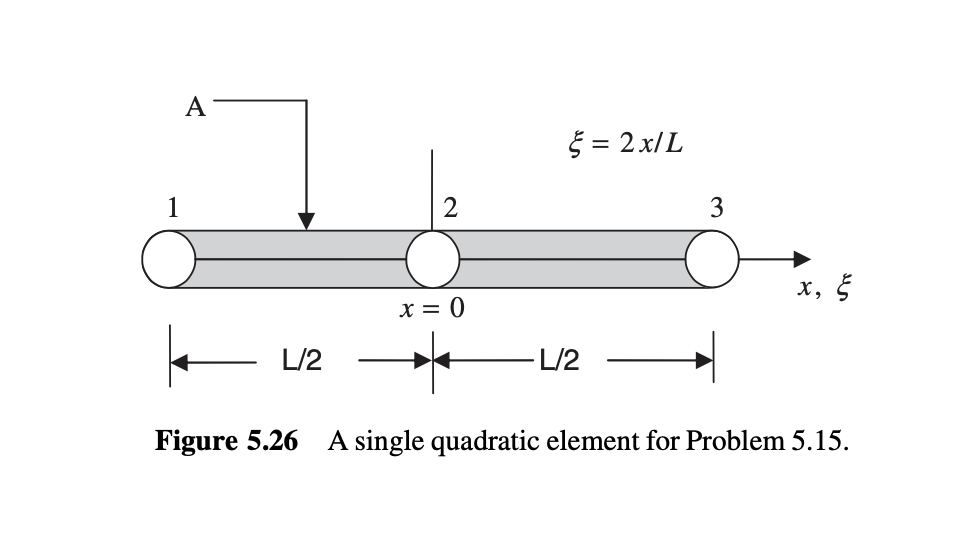
\includegraphics[width=0.5\textwidth]{figure_1.png}  % Replace with your image file name
    \caption{Problem 1}
    \label{fig:element}
\end{figure}

\begin{enumerate}
    \item[(a)] \textbf{(20 points)} Verify that if the nodes are uniformly spaced, the element Jacobian is given by \( J = \frac{L}{2} \).

    
    \item[(b)] \textbf{(20 points)} If \( \epsilon_x \) at node 1 is to remain finite, how far from the center can node 2 be moved?
 
\end{enumerate}


\subsection*{a.$)$}
 Verify that if the nodes are uniformly spaced, the element Jacobian is given by $J = \frac{L}{2}$

Note: I did most all of the math and calculated these values when I was trying to solve problem 1. I worked on the problems in order, and did not know that I would be calcuating the values that I used in problem 1 later. So in this section I restate the results and what
I did to get the values, because the math is calculated in problem 1.

\subsubsection*{Step 1: Define the Coordinates and the Mapping}
For a three-node isoparametric quadratic element with nodes located at \(\xi = -1\), \(\xi = 0\), and \(\xi = 1\), the global coordinates \( x \) at any point within the element can be expressed in terms of the shape functions and nodal coordinates \( x_1 \), \( x_2 \), and \( x_3 \) as:

\[
x(\xi) = N_1(\xi) x_1 + N_2(\xi) x_2 + N_3(\xi) x_3,
\]

where:
\begin{itemize}
    \item \( N_1(\xi) = \frac{1}{2} \xi (\xi - 1) \),
    \item \( N_2(\xi) = 1 - \xi^2 \),
    \item \( N_3(\xi) = \frac{1}{2} \xi (\xi + 1) \).
\end{itemize}

\subsubsection*{Step 2: Substitute Uniform Node Spacing}
Assume that the nodes are uniformly spaced along the length \( L \) of the element:
\begin{align*}
    x_1 &= -\frac{L}{2}, \\
    x_2 &= 0, \\
    x_3 &= \frac{L}{2}.
\end{align*}

\subsubsection*{Step 3: Calculate the Jacobian \( J = \frac{dx}{d\xi} \)}
The Jacobian \( J \) is defined as the derivative of \( x \) with respect to \( \xi \):

\[
J = \frac{dx}{d\xi}.
\]

Using the expression for \( x(\xi) \), we differentiate with respect to \( \xi \):

\[
\frac{dx}{d\xi} = \frac{dN_1}{d\xi} x_1 + \frac{dN_2}{d\xi} x_2 + \frac{dN_3}{d\xi} x_3.
\]

\subsubsection*{Step 4: Calculate Each Derivative of the Shape Functions}
Now, calculate \( \frac{dN_1}{d\xi} \), \( \frac{dN_2}{d\xi} \), and \( \frac{dN_3}{d\xi} \):

1. For \( N_1(\xi) = \frac{1}{2} \xi (\xi - 1) \):
   \[
   \frac{dN_1}{d\xi} = \frac{1}{2} (2\xi - 1) = \xi - \frac{1}{2}.
   \]

2. For \( N_2(\xi) = 1 - \xi^2 \):
   \[
   \frac{dN_2}{d\xi} = -2\xi.
   \]

3. For \( N_3(\xi) = \frac{1}{2} \xi (\xi + 1) \):
   \[
   \frac{dN_3}{d\xi} = \frac{1}{2} (2\xi + 1) = \xi + \frac{1}{2}.
   \]

\subsubsection*{Step 5: Substitute and Simplify}
Substitute these derivatives and the values of \( x_1 \), \( x_2 \), and \( x_3 \) into the Jacobian expression:

\[
J = \frac{dx}{d\xi} = \left(\xi - \frac{1}{2}\right) \left(-\frac{L}{2}\right) + (-2\xi) \cdot 0 + \left(\xi + \frac{1}{2}\right) \frac{L}{2}.
\]

Simplifying, we get:

\[
J = -\frac{L}{2} \left(\xi - \frac{1}{2}\right) + \frac{L}{2} \left(\xi + \frac{1}{2}\right).
\]

Expanding both terms:

\[
J = -\frac{L}{2} \xi + \frac{L}{4} + \frac{L}{2} \xi + \frac{L}{4}.
\]

Combine terms:

\[
J = \frac{L}{2}.
\]

\subsubsection*{Conclusion}
Thus, we have verified that the Jacobian for this uniformly spaced three-node isoparametric quadratic element is indeed \( J = \frac{L}{2} \), as required.

\newpage
\subsection*{b.$)$}
If \( \epsilon_x \) at node 1 is to remain finite, how far from the center can node 2 be moved?


\subsubsection*{1. Displacement Field and Strain for a Quadratic Element}
I did this in problem 1 too, so I will just quickly restate the values that I calculated from that problem.\\

For a three-node isoparametric quadratic element, the displacement field \( u(x) \) in terms of the natural coordinate \( \xi \) and nodal displacements \( u_1 \), \( u_2 \), and \( u_3 \) is:

\[
u(\xi) = N_1(\xi) u_1 + N_2(\xi) u_2 + N_3(\xi) u_3,
\]

where:
- \( N_1(\xi) = \frac{1}{2} \xi (\xi - 1) \),
- \( N_2(\xi) = 1 - \xi^2 \),
- \( N_3(\xi) = \frac{1}{2} \xi (\xi + 1) \).

The strain \( \epsilon_x \) is the derivative of the displacement with respect to \( x \):

\[
\epsilon_x = \frac{du}{dx}.
\]

Since we are working in terms of \( \xi \), we use the chain rule:

\[
\epsilon_x = \frac{du}{d\xi} \cdot \frac{d\xi}{dx}.
\]

\subsubsection*{2. Derivative of \( u \) with Respect to \( \xi \)}

Taking the derivative of \( u(\xi) \) with respect to \( \xi \):

\[
\frac{du}{d\xi} = \frac{dN_1}{d\xi} u_1 + \frac{dN_2}{d\xi} u_2 + \frac{dN_3}{d\xi} u_3.
\]

Using the derivatives of the shape functions:
- \( \frac{dN_1}{d\xi} = \xi - \frac{1}{2} \),
- \( \frac{dN_2}{d\xi} = -2\xi \),
- \( \frac{dN_3}{d\xi} = \xi + \frac{1}{2} \),

we can write:

\[
\frac{du}{d\xi} = \left( \xi - \frac{1}{2} \right) u_1 - 2\xi u_2 + \left( \xi + \frac{1}{2} \right) u_3.
\]

\subsubsection*{3. Jacobian \( \frac{d\xi}{dx} \)}

The Jacobian \( J = \frac{dx}{d\xi} \) for this element maps between the natural coordinate \( \xi \) and the physical coordinate \( x \):

\[
\frac{dx}{d\xi} = \frac{dN_1}{d\xi} x_1 + \frac{dN_2}{d\xi} x_2 + \frac{dN_3}{d\xi} x_3.
\]

Substituting \( x_1 \), \( x_2 \), and \( x_3 \), and using the derivatives of the shape functions, we get:

\[
\frac{dx}{d\xi} = \left( \xi - \frac{1}{2} \right) x_1 - 2\xi x_2 + \left( \xi + \frac{1}{2} \right) x_3.
\]

The strain \( \epsilon_x \) becomes:

\[
\epsilon_x = \frac{du}{d\xi} \cdot \frac{1}{\frac{dx}{d\xi}}.
\]

\subsubsection*{4. Behavior of \( \frac{dx}{d\xi} \) as Node 2 Approaches Node 1 or Node 3}

1. If node 2 approaches node 1:\\
   - As \( x_2 \) approaches \( x_1 \), the distance between nodes 1 and 2 shrinks.\\
   - In this case, the terms involving \( x_1 \) and \( x_2 \) in \( \frac{dx}{d\xi} \) nearly cancel each other out, making \( \frac{dx}{d\xi} \) very small.\\
   - Since \( \epsilon_x = \frac{du}{d\xi} \cdot \frac{1}{\frac{dx}{d\xi}} \), a small \( \frac{dx}{d\xi} \) in the denominator causes \( \epsilon_x \) to become very large.\\

2. If node 2 approaches node 3:\\
   - Similarly, as \( x_2 \) approaches \( x_3 \), the distance between nodes 2 and 3 shrinks.\\
   - This causes the terms involving \( x_2 \) and \( x_3 \) in \( \frac{dx}{d\xi} \) to nearly cancel out, again making \( \frac{dx}{d\xi} \) very small.\\
   - With \( \frac{dx}{d\xi} \) small, the strain \( \epsilon_x \) again becomes large due to division by a small number.\\

\subsubsection*{Conclusion}

To keep \( \epsilon_x \) finite, node 2 must stay far from nodes 1 and 3 to avoid \( \frac{dx}{d\xi} \) approaching zero. Moving node 2 too close to either node 1 or node 3 leads to strain approaching infinity. 
So, node 2 should remain within a certain range around the center for the strain to remain finite.

The distance \( x_2 \) from the center should remain within \( -\frac{L}{2} < x_2 < \frac{L}{2} \), with \( x_2 \) ideally not too close to either boundary.


%%%%%%%%%%%%%%%%%%%%%%%%%%%%%%%%
%%%%%%%%%%%%%%%%%%%%%%%%%%%%%%%%%%%

\newpage
\section*{Problem 3}

Show that the subparametric triangular element (defined by combining quadratic 6-noded shape functions for the trial solution approximation with the linear map given in Eq. (7.47) in the text) is:
\begin{enumerate}
    \item[(a)] (15 points) \textbf{Linear Complete:} Demonstrate that the element can represent any linear function exactly.
    \item[(b)] (10 points) \textbf{Quadratic Field Representation:} Prove that the element is capable of exactly representing the quadratic field \( x^2 \).
\end{enumerate}

Equation (7.47) in the text is given by:
\[
x = \sum_{I=1}^{3} x_I^e \xi_I, \quad y = \sum_{I=1}^{3} y_I^e \xi_I.
\]

\subsection*{a.$)$}
Demonstrate that the element can represent any linear function exactly.

I want to demostrate that the shape functions for the 6-node element can exactly represent any linear field (they can reproduce x and y exactly).
The textbook solves this for the three node element, so I want to use that same approach for a 6 node element.

\subsubsection*{Define Linear Field}
the field $\theta(x,y)$ is linear if it is in the form:

\begin{equation}
    \theta(x,y) = \alpha_0 + \alpha_1 x + \alpha y
    \label{eq:linear}
\end{equation}

\subsubsection*{Shape Functions for a 6-Node Triangle Element}
Table 7.5 gives us the values of the Shape Functions:
\[
    N_1 = \xi_1 (2 \xi_1 -1)
\]
\[
    N_2 = \xi_2 (2 \xi_2 -1)
\]
\[
    N_3 = \xi_3 (2 \xi_3 -1)
\]
\[
    N_4 = 4\xi_1\xi_2
\]
\[
    N_5 = 4\xi_2\xi_3
\]
\[
    N_6 = 4\xi_1\xi_3
\]

\subsubsection*{Use the Interpolated Function}
The isoparametric element is defined using equations (7.53) in the textbook. We can use the approximation as:

\begin{equation}
    \theta^{e}(\xi) = \sum_{i=1}^{6} \theta_I N_I^{6L}(\xi)
    \label{eq:sum}
\end{equation}

we want to show that if the nodal values are set by:
\begin{equation}
    \theta_I = \alpha_0 + \alpha_1 x_I
    \label{eq:theta}
\end{equation}

and we can substitute \ref{eq:theta} into \ref{eq:sum}:

\begin{equation*}
    \theta(x,y) = \sum_{I=1}^{6} (\alpha_0 + \alpha_1 x +\alpha_2 y) {N_I}^{6L}(\xi)
\end{equation*}

so when we expand this over the 6 nodes we have:

\begin{equation*}
    \theta(x,y) = \alpha_0 + \alpha_1 \sum_{I=1}^{6}N_I^{6L}(\xi)(x_I) +\alpha_2 \sum_{I=1}^{6}N_I^{6L}(\xi)(y_I) 
\end{equation*}

Equation (7.47) from the text is in the above equation. But the partition of unity property states
\[
    \sum_{I=1}^{6} N_{I}^{6L}(\xi) = 1
\]

so the equation simplifies to:

\begin{equation*}
    \theta(x,y) = \alpha_0 + \alpha_1 x_I +\alpha_2 y_I
\end{equation*}

which matches the linear equation \ref{eq:linear} proving the 6 node element is linear complete.

\newpage
\subsubsection*{b.$)$}
Prove that the element is capable of exactly representing the quadratic field \( x^2 \)

I can apply a similar approach to the quadratic in this case that I did for the linear.

\subsubsection*{Define Quadratic Field}
Using the pascal triangle we can say the field $\theta(x,y)$ is quadratic if it is in the form:

\begin{equation}
    \theta(x,y) = \alpha_0 + \alpha_1 x_I^2 + \alpha_2 x_I y_I + \alpha_3 y_I^2
    \label{eq:quadratic}
\end{equation}

\subsubsection*{Shape Functions for a 6-Node Triangle Element}
Table 7.5 gives us the values of the Shape Functions:
\[
    N_1 = \xi_1 (2 \xi_1 -1)
\]
\[
    N_2 = \xi_2 (2 \xi_2 -1)
\]
\[
    N_3 = \xi_3 (2 \xi_3 -1)
\]
\[
    N_4 = 4\xi_1\xi_2
\]
\[
    N_5 = 4\xi_2\xi_3
\]
\[
    N_6 = 4\xi_1\xi_3
\]

\subsubsection*{Use the Interpolated Functio}
The isoparametric element is defined using equations (7.53) in the textbook. We can use the approximation as:

\begin{equation}
    \theta^{e}(\xi) = \sum_{i=1}^{6} \theta_I N_I^{6L}(\xi)
    \label{eq:qsum}
\end{equation}

we want to show that if the nodal values are set by:
\begin{equation}
    \theta_I = \alpha_0 + \alpha_1 x_I
    \label{eq:theta}
\end{equation}

and we can substitute \ref{eq:quadratic} into \ref{eq:qsum}:

\begin{equation*}
    \theta(x,y) = \sum_{I=1}^{6} (\alpha_0 + \alpha_1 x^2 +\alpha_2 x y + \alpha_3 y^2) {N_I}^{6L}(\xi)
\end{equation*}

so when we expand this over the 6 nodes we have:

\begin{equation*}
    \theta(x,y) = \alpha_0 + \alpha_1 \sum_{I=1}^{6}N_I^{6L}(\xi)(x_I^2) +\alpha_2 \sum_{I=1}^{6}N_I^{6L}(\xi)(x_I y_I)  + \alpha_3 \sum_{I=1}^{6}N_I^{6L}(\xi)(y_I^2)
\end{equation*}

Equation (7.47) from the text is in the above equation. But the partition of unity property states
\[
    \sum_{I=1}^{6} N_{I}^{6L}(\xi) = 1
\]

so the equation simplifies to:

\begin{equation*}
    \theta(x,y) = \alpha_0 + \alpha_1 x_I^2 +\alpha_2 x_I y_I + \alpha_3 y_I^2
\end{equation*}

which matches the quadratic equation \ref{eq:quadratic} proving the 6 node element represents the quadratic field.

\end{document}

